\subsection{DETAILS OF THE DIAGNOSTIC X-RAY EQUIPMENT}

\begin{table}[H]
	\centering
	\setlength{\arrayrulewidth}{1.2pt}
	\renewcommand{\arraystretch}{1.4}
	\begin{tabular}{|p{0.45\textwidth}|p{0.45\textwidth}|}
		\hline
		\textbf{Name of the Institution and City} & NISER Health Center, Jatani \\
		\hline
		\textbf{Type of Equipment} & Medical X-Ray Collimator \\
		\hline
		\textbf{Model Name} & SR-102 \\
		\hline
		\textbf{Name of the Manufacturer} & Hangzhou Sailray Imp \& Exp Co. Ltd \\
		\hline
		\textbf{Name(s) of Person(s) testing the equipment} & Souvik Das and Deepak Saini \\
		\hline
		\textbf{Dates and Duration of the Tests} & 08/01/2026, in 2 days \\
		\hline
	\end{tabular}
\end{table}

\subsection{CONGRUENCE OF RADIATION \& OPTICAL FIELD}

\begin{figure}[H]
    \centering
    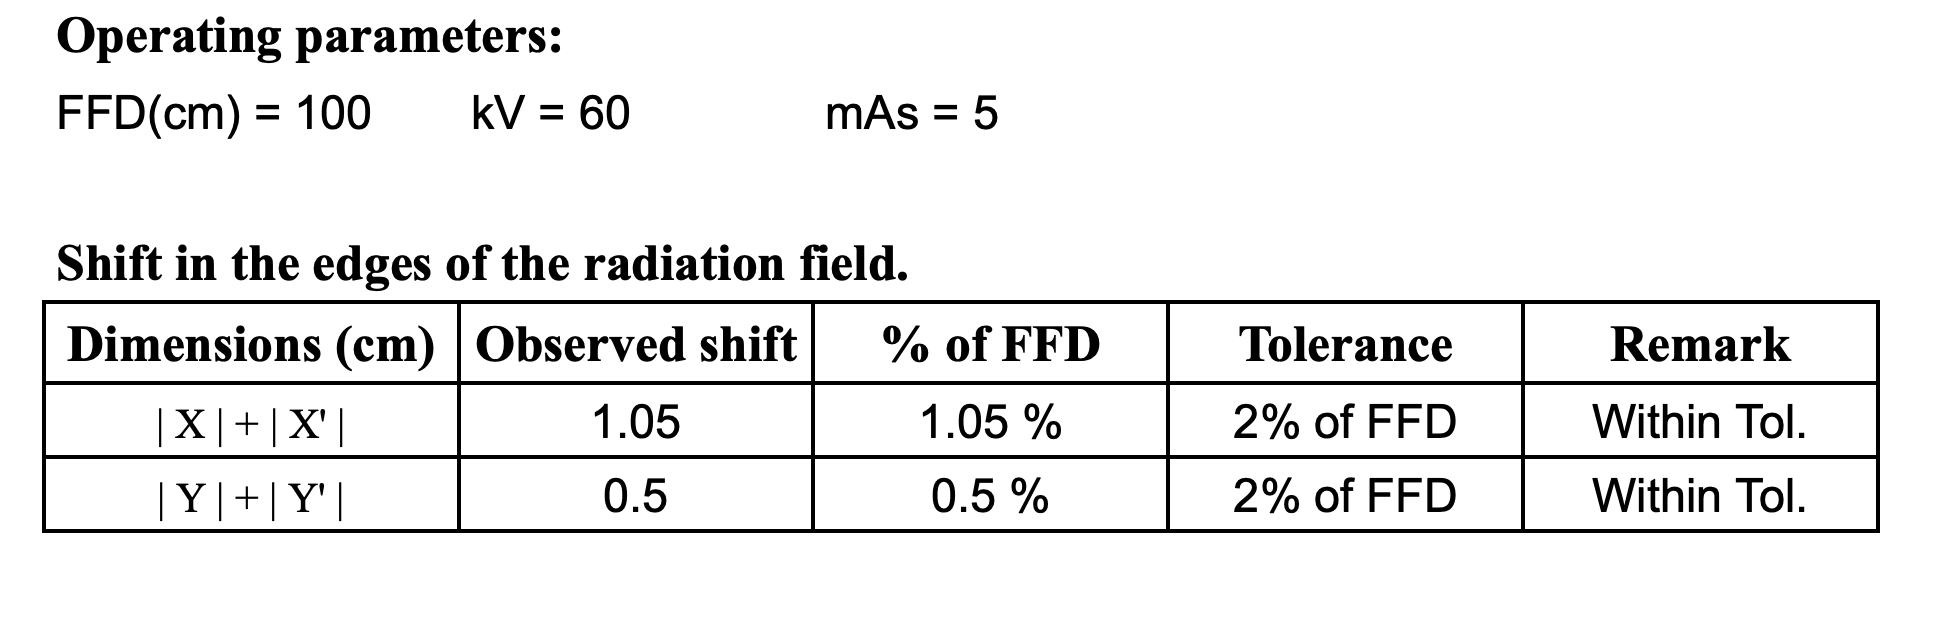
\includegraphics[width=0.7\textwidth]{Figures/Experimental_Figures/OpticalField.png}
\end{figure}

\begin{figure}[H]
	\centering
	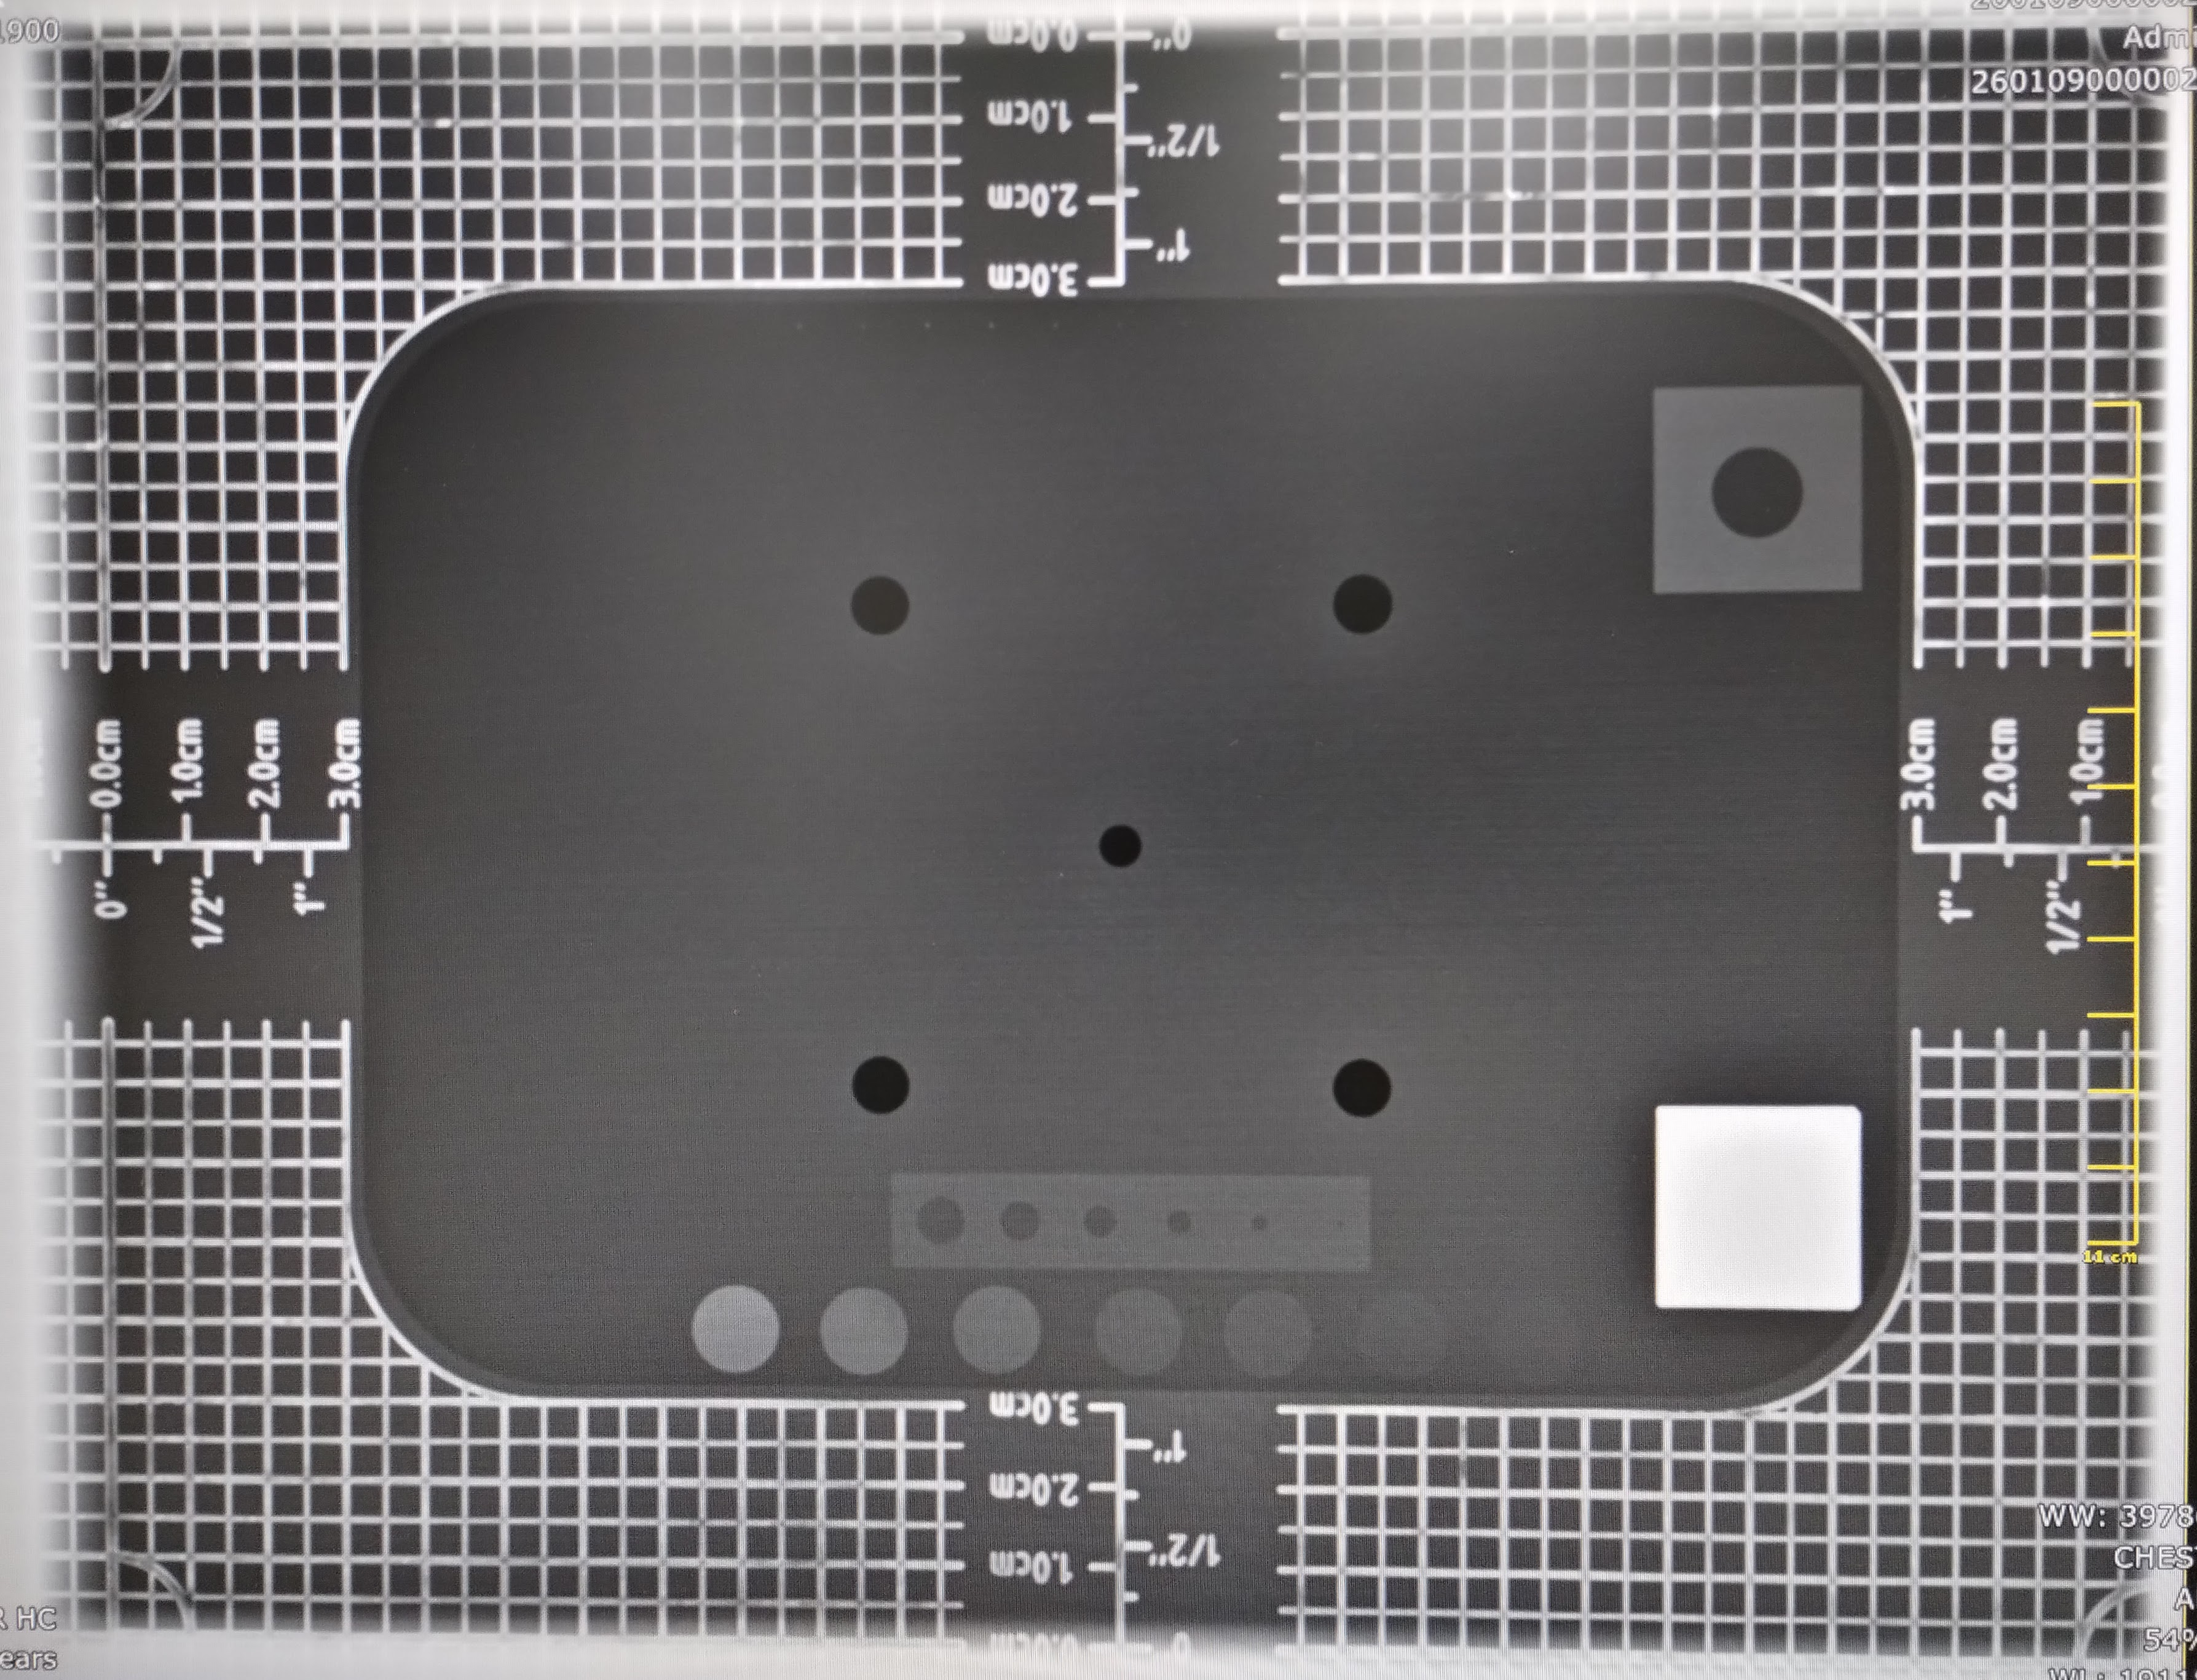
\includegraphics[width=0.5\textwidth]{Figures/Experimental_Figures/FieldCongruence.jpg}
	\caption{X-ray image of Pro-RF basic phantom.}
\end{figure}
\subsection{CENTRAL BEAM ALIGNMENT}
\begin{figure}[H]
    \centering
    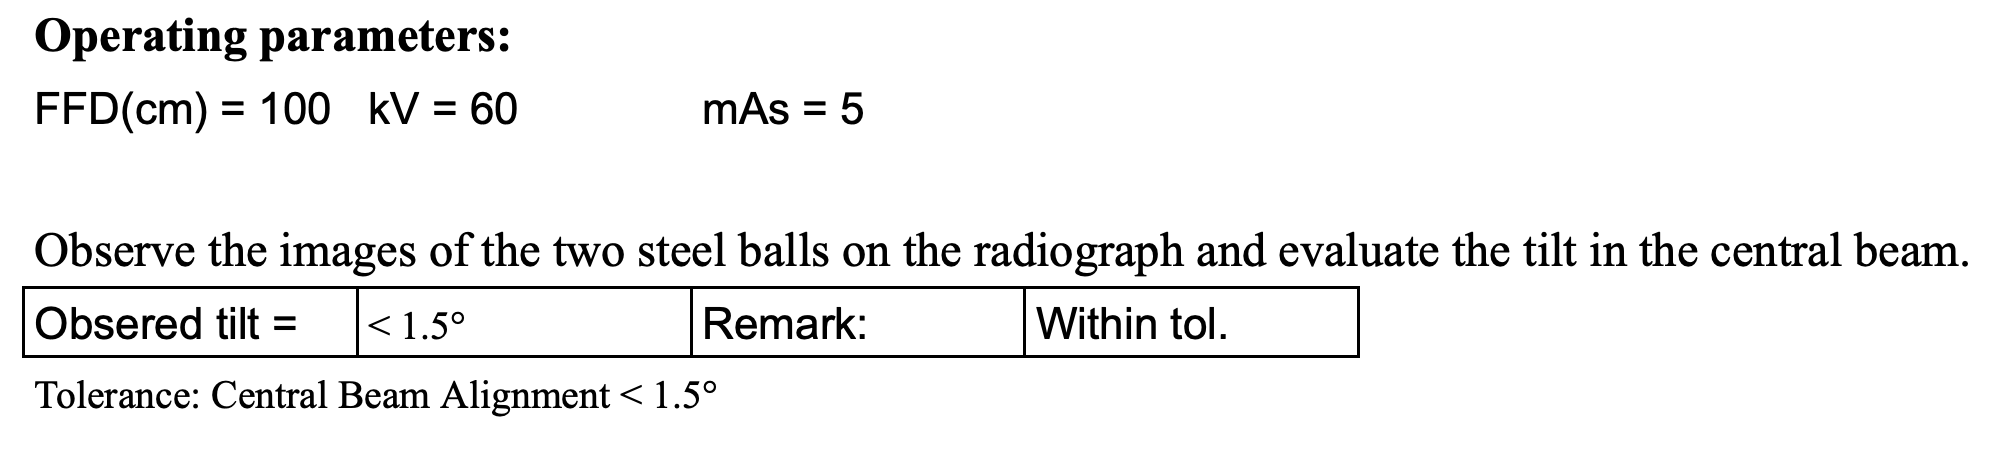
\includegraphics[width=0.9\textwidth]{Figures/Experimental_Figures/CentralBeamAllingment.png}
\end{figure}
\begin{figure}[H]
    \centering
    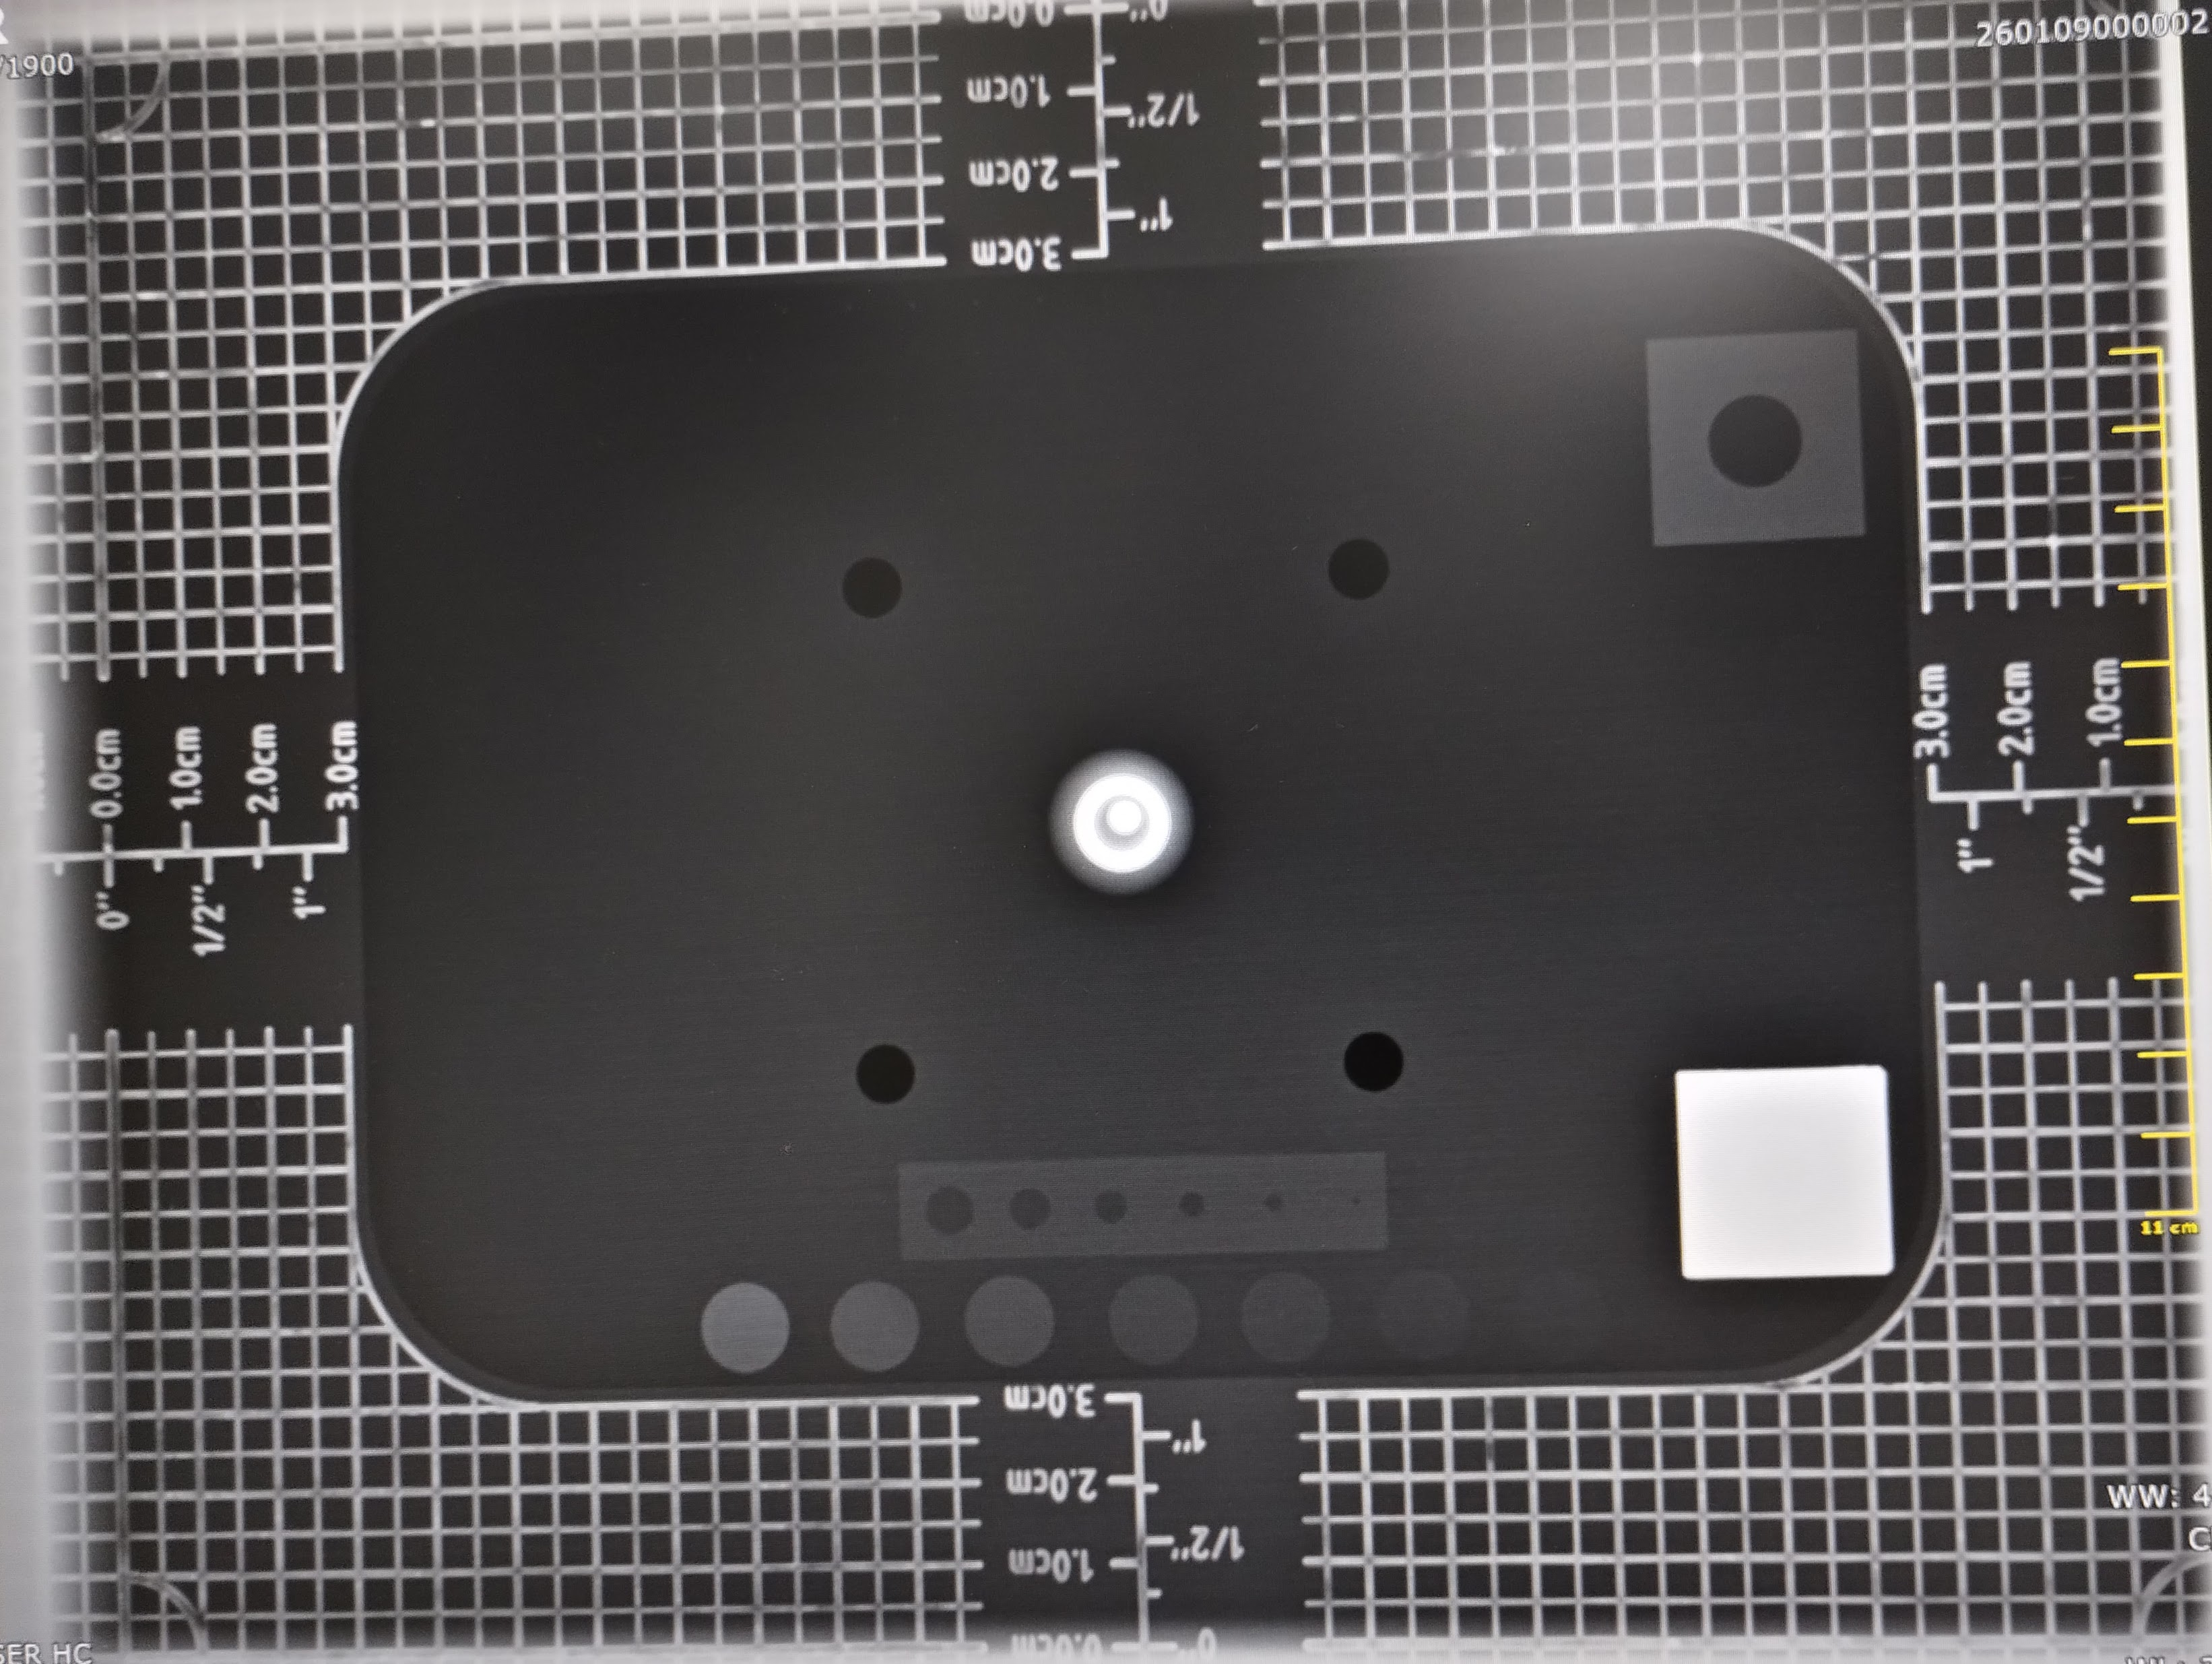
\includegraphics[width=0.45\textwidth]{Figures/Experimental_Figures/CentralAxisallignment.jpg}
	\caption{Verification of central beam alignment using cone test.}
\end{figure}
\subsection{EFFECTIVE FOCAL SPOT MEASUREMENT}
\begin{figure}[H]
	\centering
	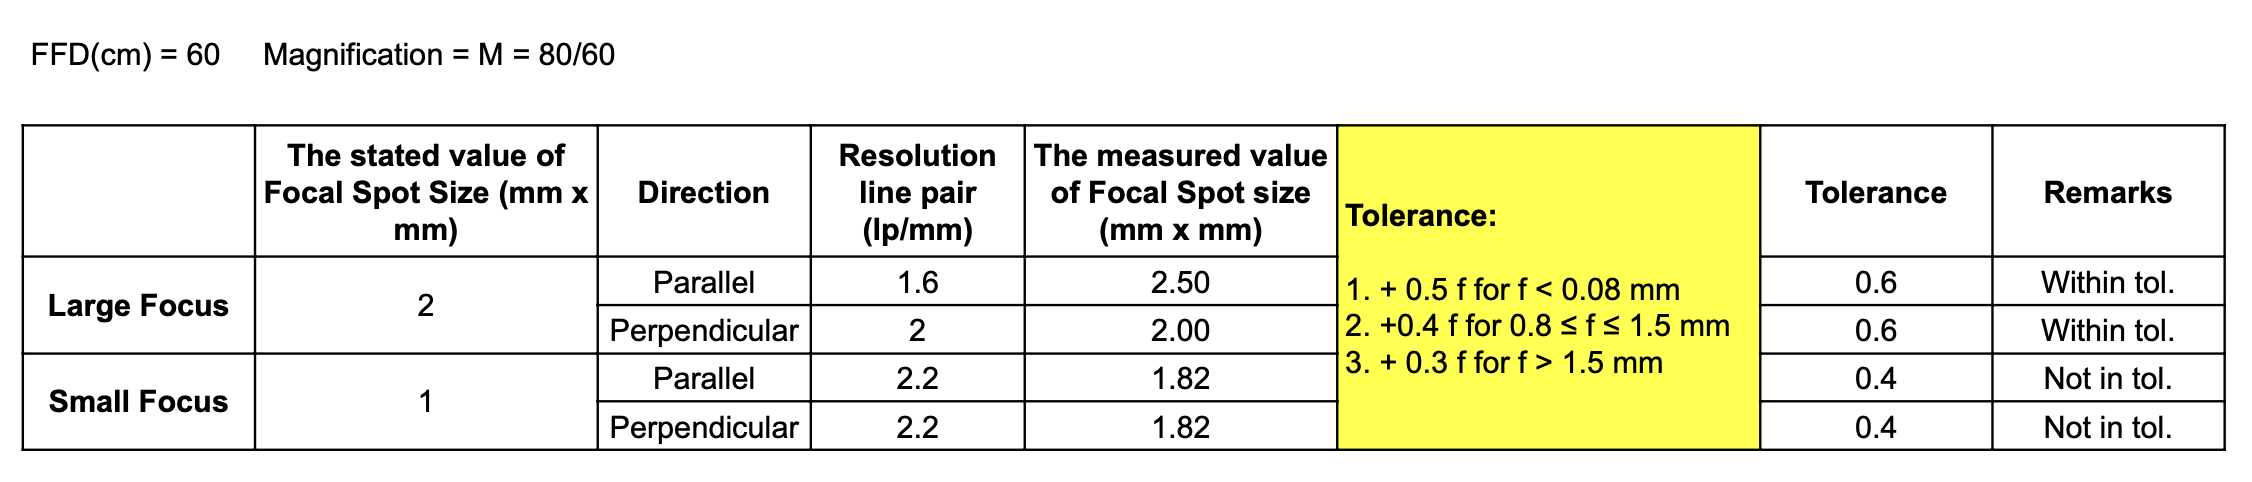
\includegraphics[width=0.9\textwidth]{Figures/Experimental_Figures/FocalSpotMeasurment.png}
\end{figure}
% two images side by side using minipage
\begin{figure}[H]
	\centering
	\begin{minipage}{0.45\textwidth}
		\centering
		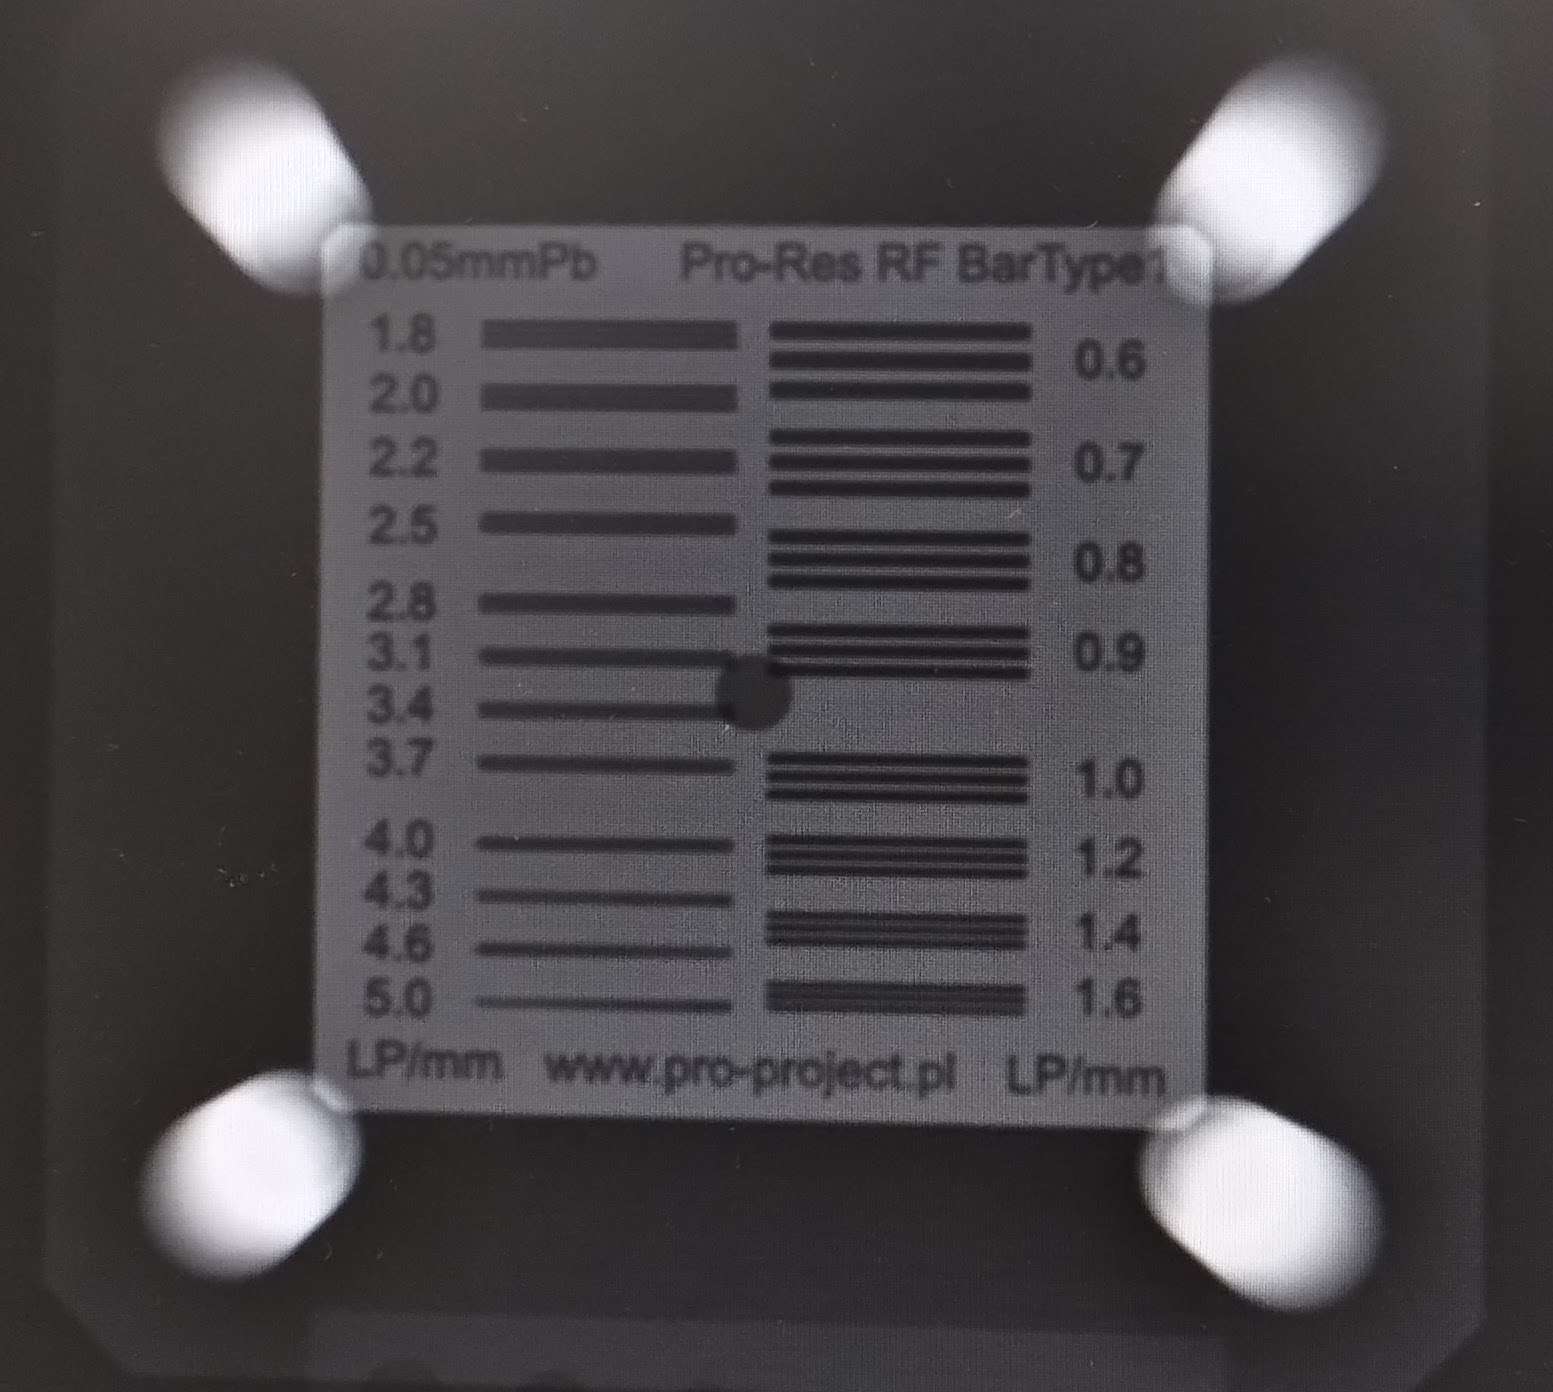
\includegraphics[width=\textwidth]{Figures/Experimental_Figures/Parallel.jpg}
		\caption{Parallel to the anode-cathode axis}
	\end{minipage}
	\hfill
	\begin{minipage}{0.37\textwidth}
		\centering
		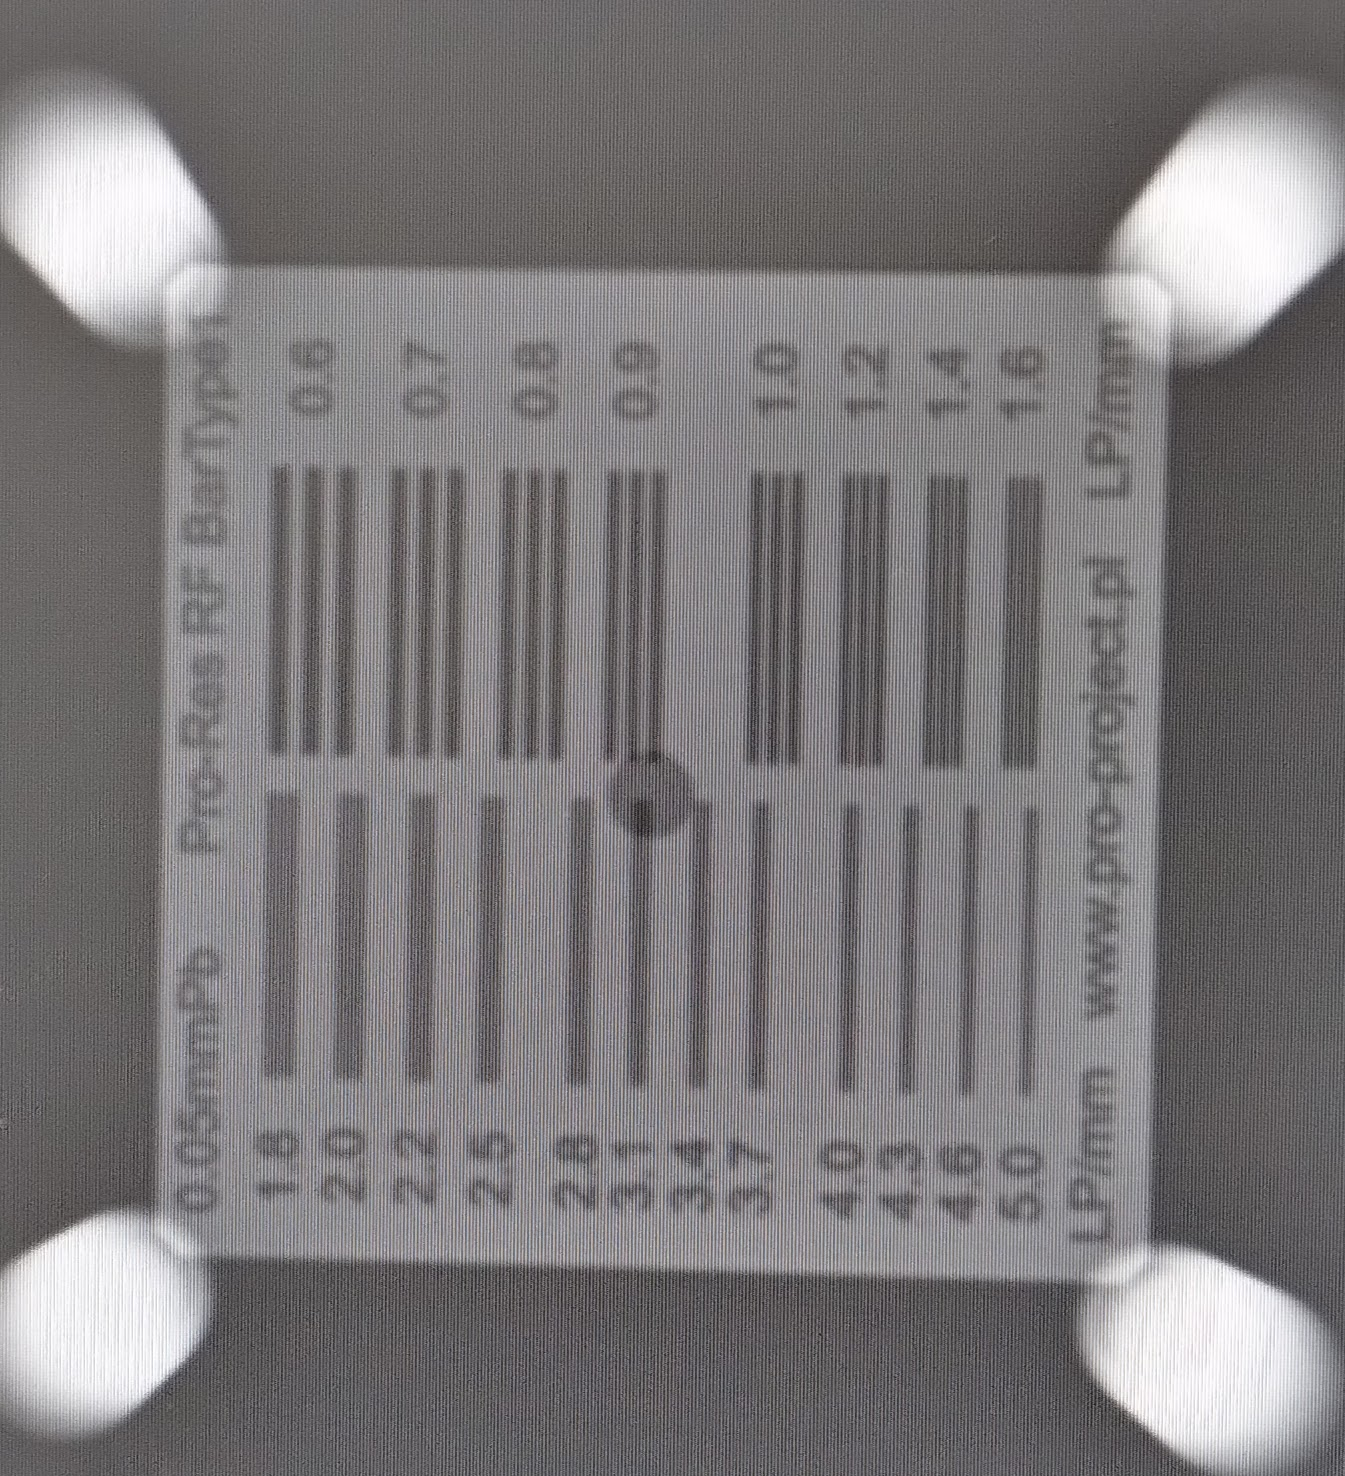
\includegraphics[width=\textwidth]{Figures/Experimental_Figures/Perpendicular.jpg}
		\caption{Perpendicular to the anode-cathode axis}
	\end{minipage}
\end{figure}


\subsection{ACCURACY OF OPERATING POTENTIAL}
\begin{figure}[H]
    \centering
    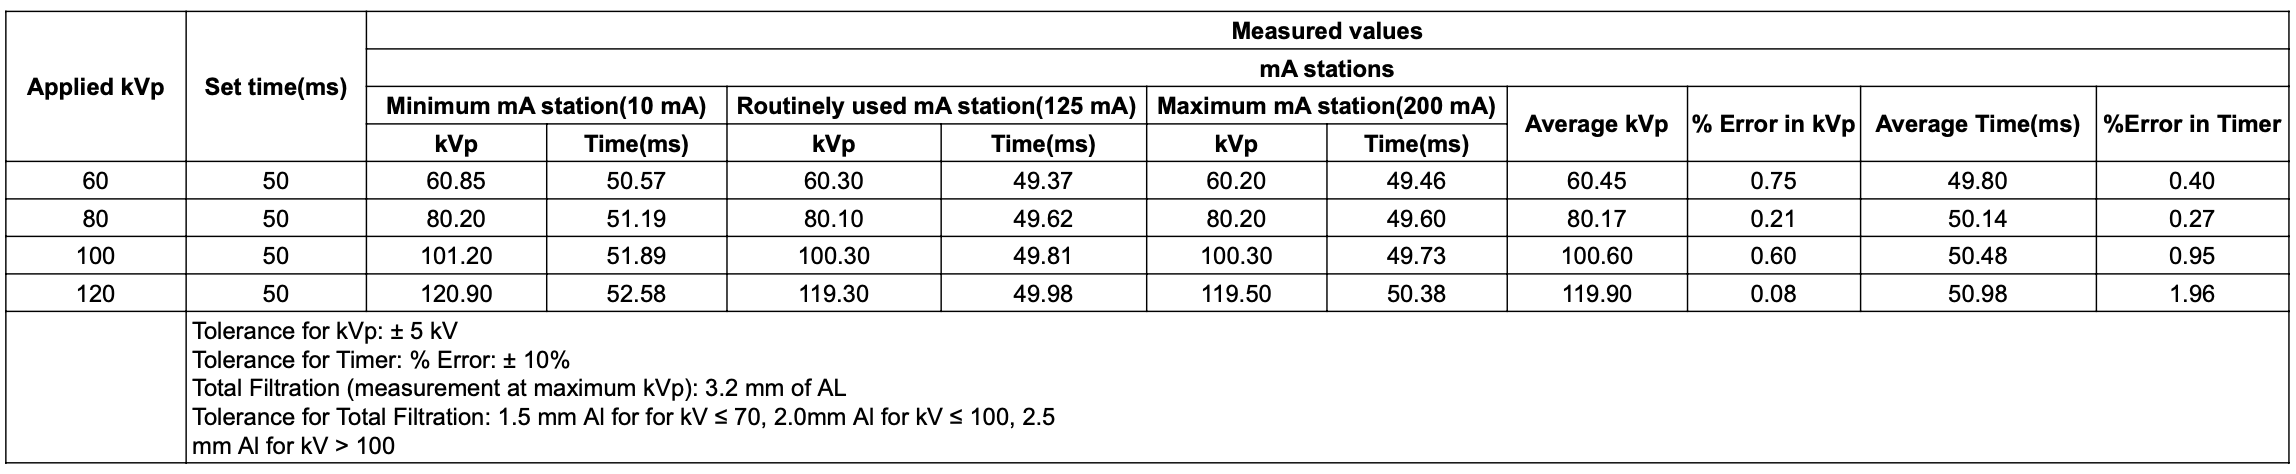
\includegraphics[width=0.9\textwidth]{Figures/Experimental_Figures/AccuracyOperatingPotential.png}
\end{figure}
So both the kVp and mAs are within the acceptable limits.
\subsection{LINEARITY OF (mA/mAs) LOADING STATIONS}
\begin{figure}[H]
    \centering
    
\includegraphics[width=0.9\textwidth]{Figures/Experimental_Figures/Linearity.png}
\end{figure}
\begin{figure}[H]
    \centering
    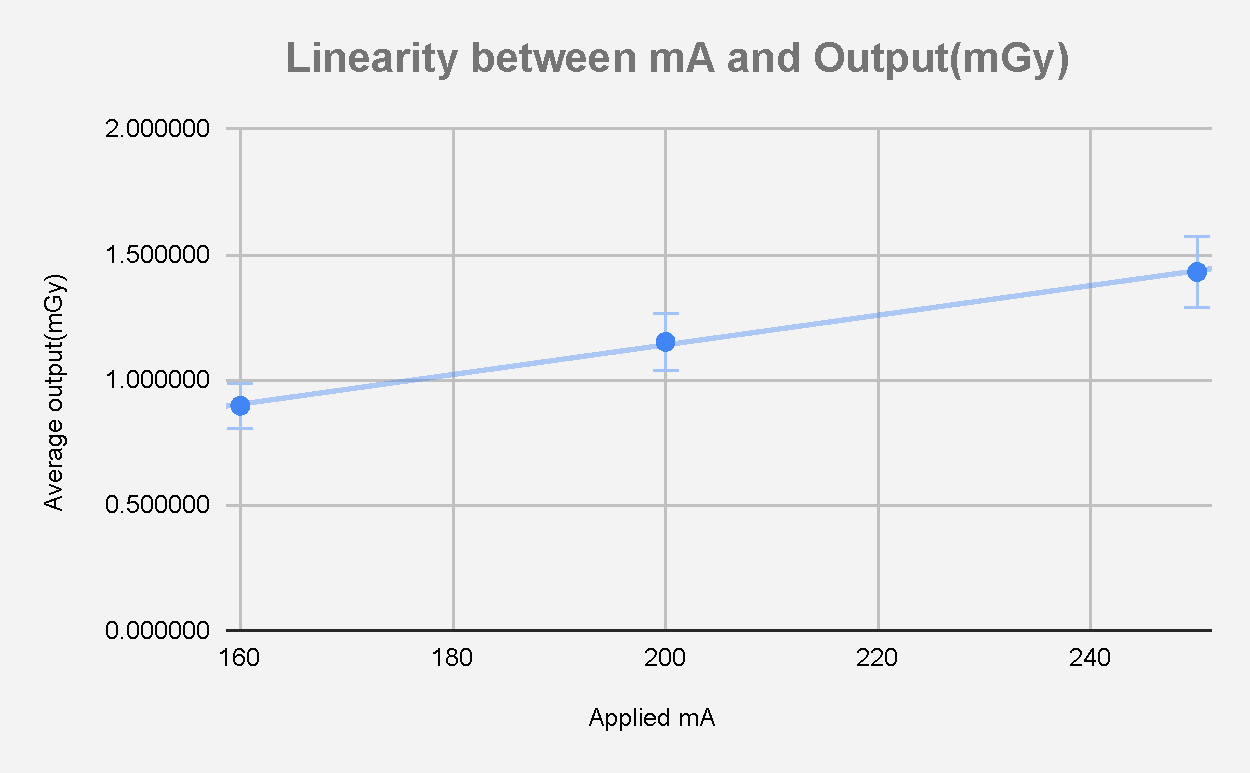
\includegraphics[width=0.6\textwidth]{Figures/Experimental_Figures/Linearity between mA and Output(mGy).pdf}
\end{figure}
\subsection{OUTPUT CONSISTENCY}
\begin{figure}[H]
    \centering
    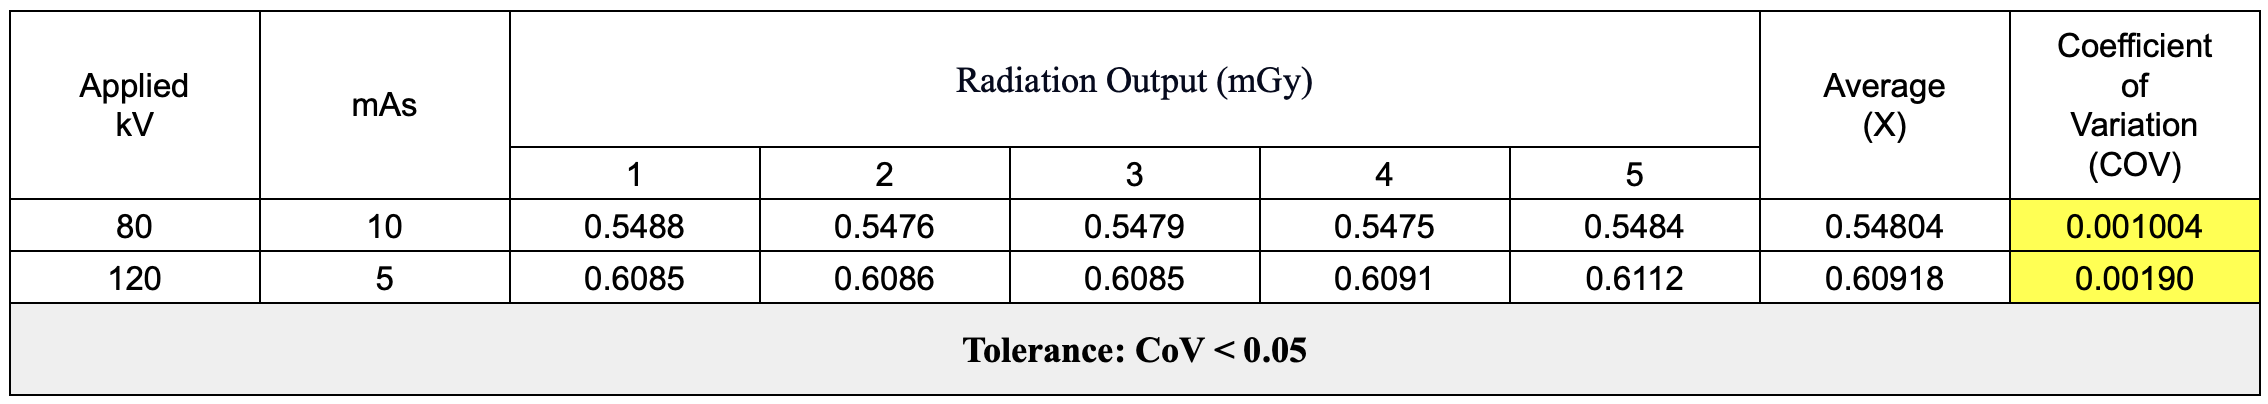
\includegraphics[width=0.9\textwidth]{Figures/Experimental_Figures/Output.png}
\end{figure}
\subsection{Contrast sensitivity}
\begin{figure}[H]
    \centering
    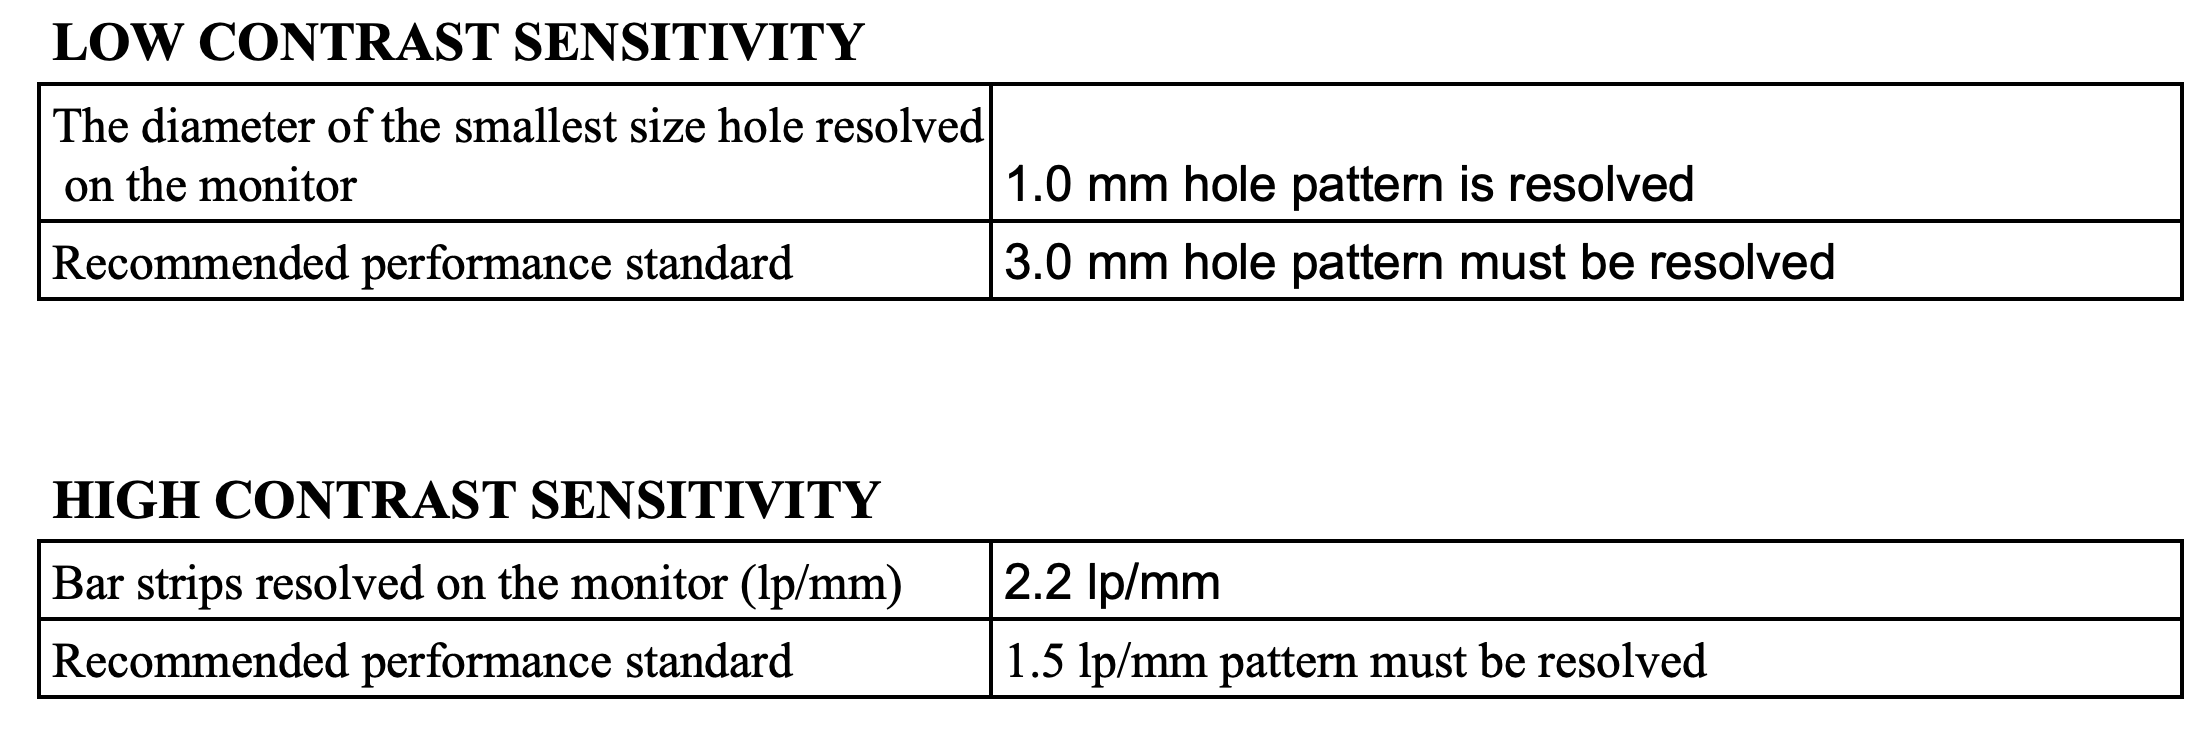
\includegraphics[width=0.9\textwidth]{Figures/Experimental_Figures/Constrast sensitivity.png}
\end{figure}
\subsection{TUBE HOUSING LEAKAGE}
\begin{figure}[H]
    \centering
    \includegraphics[width=0.9\textwidth]{Figures/Experimental_Figures/TubeHousing Leakage.png}
\end{figure}
Work load = 180 mA-min in one hour.
\begin{align*}
	\text{Leakage radiation in one hour} &= \frac{\text{180 mAmin in 1hr} \times \text{Max Exposure level (mG/hr)}}{60 \times \text{mA used for measurement}}\\
\end{align*}
Maximum radiation leakage from tube housing = \textbf{131.64} $\mu$Gy/hr. And maximum radiation leakage from tube collimator = \textbf{0.19872} $\mu$Gy/hr.


\subsection{DETAILS OF RADIATION PROTECTION SURVEY OF THE INSTALLATION}
kVp = 120,	mA =100 and	time = 1 s.
\begin{figure}[H]
	\centering
	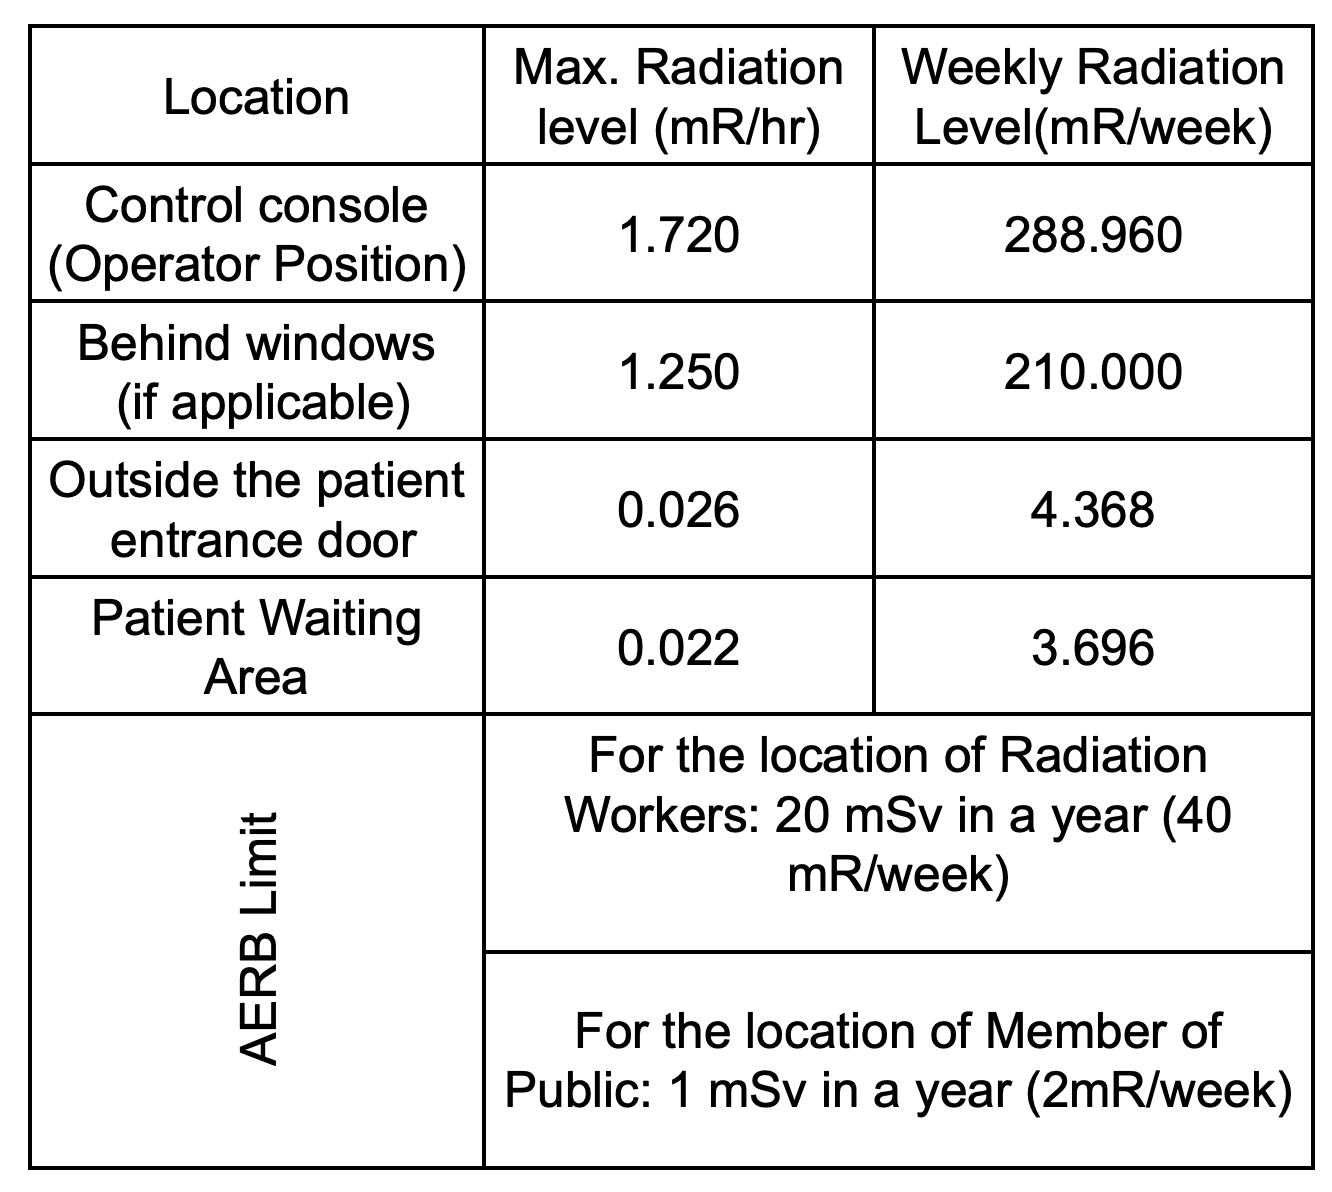
\includegraphics[width=0.45\textwidth]{Figures/Experimental_Figures/Radiation protection.png}
\end{figure}
